% Variation diagram: a function f(x) (blue) and a varied function
% \tilde f(x) (red, dot-dashed) sharing the same endpoints A, B, with the
% pointwise variation \delta f(x) shown by dotted green segments.
%
% Compile standalone with:  pdflatex 变分f_tikz.tex
\documentclass[tikz,border=6pt]{standalone}
\usepackage{amsmath}
\usetikzlibrary{arrows.meta, calc}

\begin{document}
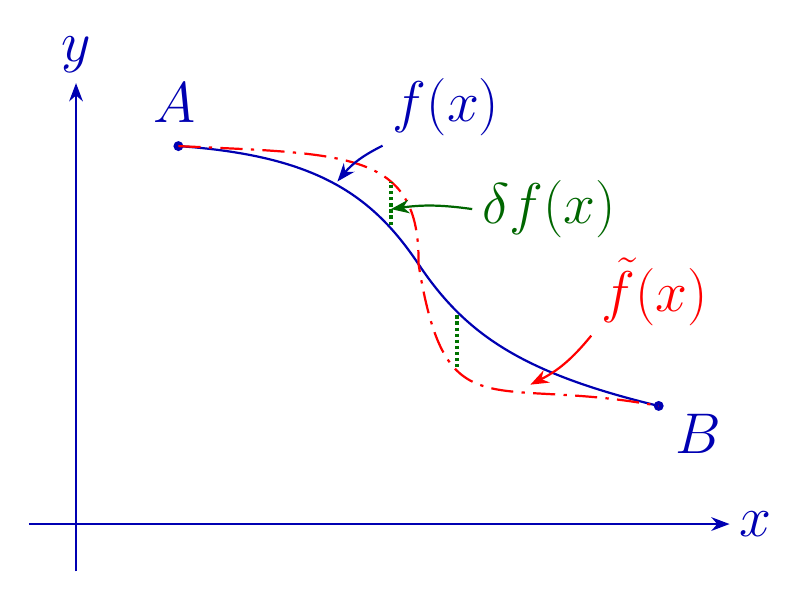
\begin{tikzpicture}[>=Stealth, thick, every node/.style={font=\fontsize{20}{24}\selectfont}]

  % ---- geometry -----------------------------------------------------
  \def\Ax{1.3} \def\Ay{4.8}
  \def\Bx{7.4} \def\By{1.5}

  % ---- axes (blue) ----------------------------------------------------
  \draw[blue!70!black, ->] (-0.6,0) -- (8.3,0) node[right] {$x$};
  \draw[blue!70!black, ->] (0,-0.6) -- (0,5.6) node[above] {$y$};

  % ---- endpoints ------------------------------------------------------
  \fill[blue!70!black] (\Ax,\Ay) circle (1.8pt);
  \fill[blue!70!black] (\Bx,\By) circle (1.8pt);
  \node[blue!70!black] at ($(\Ax,\Ay)+(-0.05,0.55)$) {$A$};
  \node[blue!70!black] at ($(\Bx,\By)+(0.5,-0.35)$) {$B$};

  % ---- the two curves ---------------------------------------------------
  % Cubic Bezier segments keep the construction compatible with the editor.
  % Both curves pass through the common midpoint (4.35,3.30).
  \draw[blue!70!black]
    (\Ax,\Ay) .. controls (3.05,4.68) and (3.76,4.18) .. (4.35,3.30)
    .. controls (4.94,2.42) and (5.65,1.92) .. (\Bx,\By);
  \draw[red, dash pattern=on 8pt off 3pt on 1.2pt off 3pt]
    (\Ax,\Ay) .. controls (3.45,4.70) and (4.37,4.74) .. (4.35,3.30)
    .. controls (4.7,1.15) and (5.25,1.90) .. (\Bx,\By);

  % ---- \delta f(x) segments between the two curves -------------------------
  \draw[green!45!black, densely dotted, line width=1.2pt]
    (4,3.8) -- (4,4.35);
  \draw[green!45!black, densely dotted, line width=1.2pt]
    (4.84,2.65) -- (4.84,2);

  % ---- labels with pointer arrows ---------------------------------------
  \node[blue!70!black] at (4.7,5.3) (flabel) {$f(x)$};
  \draw[blue!70!black, ->] (flabel.south west) to[bend right=12] (3.32,4.35);

  \node[red] at (7.35,2.95) (ftlabel) {$\tilde f(x)$};
  \draw[red, ->] (ftlabel.south west) to[bend left=12] (5.77,1.77);

  \node[green!40!black] at (6.01,4) (dflabel) {$\delta f(x)$};
  \draw[green!40!black, ->] (dflabel.west) to[bend right=8] (4,4);

\end{tikzpicture}
\end{document}
